\documentclass[../../tc_tp5_main.tex]{subfiles}

\begin{document}

%capítulo
\chapter{Celda Rauch (Deliyannis-Friend modificada)}
Se busca implementar un filtro pasabanda con las siguientes especificaciones:\par

\begin{figure}[H]	%especificaciones Rauch consigna
	\centering
	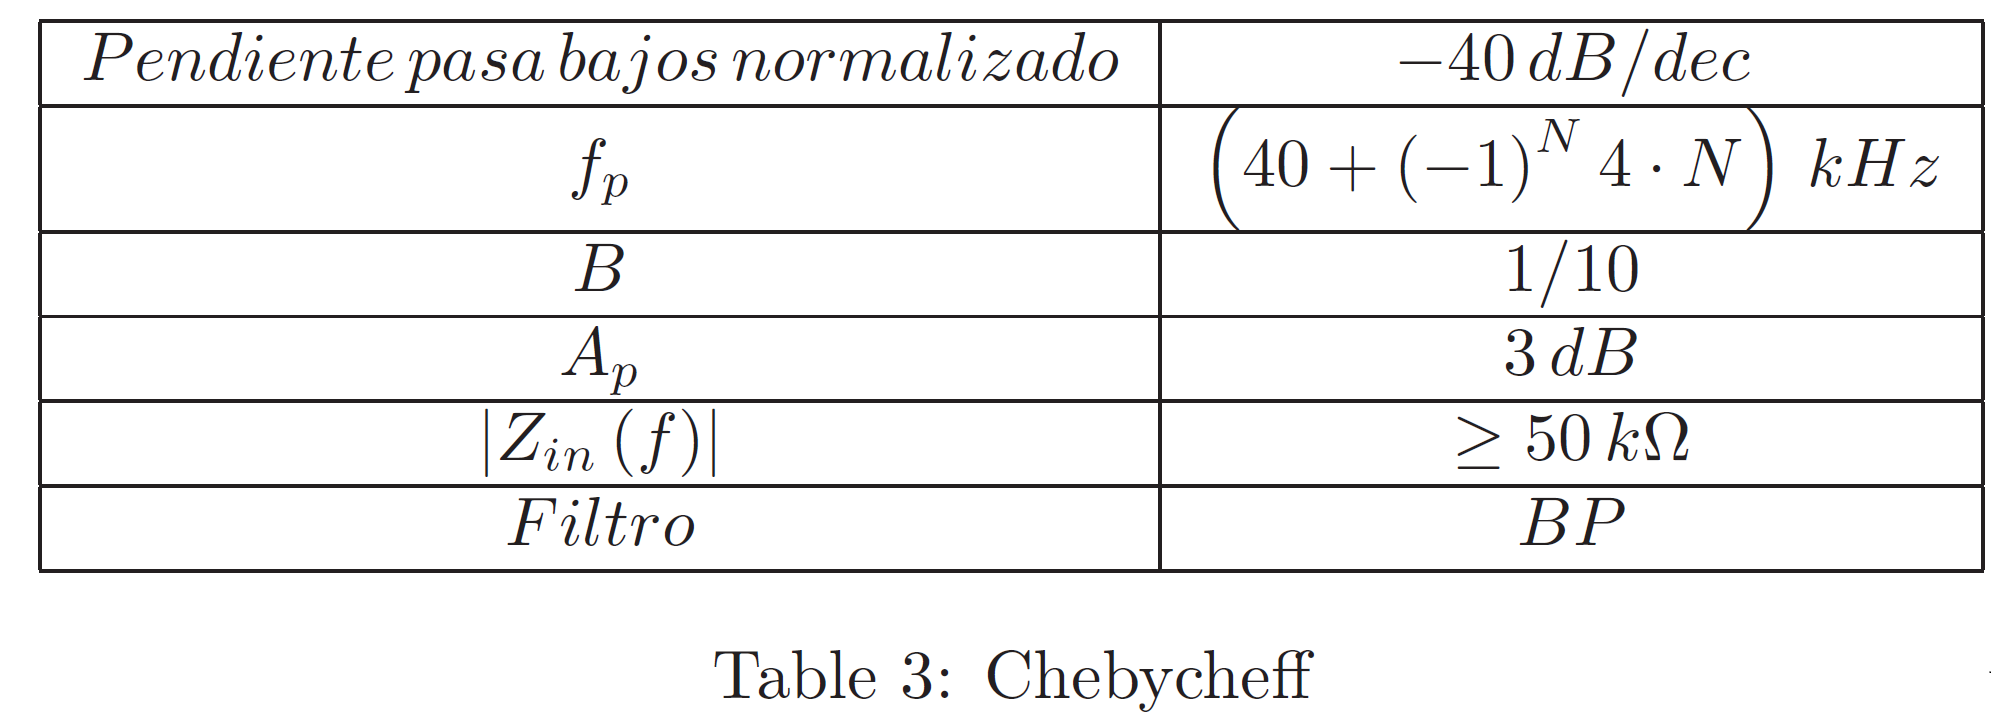
\includegraphics[scale=0.5]{imagenes/especificaciones.png}
	\caption{Especificaciones del filtro pedido por consigna}
	\label{fig:ej2_especificaciones}
\end{figure}

De estas especificaciones, dado que la pendiente del pasabajos normalizado es de 40dB/década, se deduce que este pasabajos es de orden 2, y por ende filtro resultante de la aproximación luego de desnormalizar será de orden 4. \par
Como la aproximación utilizada será Chevyshev, los 2 polos obtenidos para el pasabajos normalizado serán polos complejos conjugados, y luego al aplicar el cambio de variable para realizar la desnormalización, la función transferencia desnormalizada estará compuesta enteramente por polos complejos conjugados y 2 ceros en el origen.\par
Se puede demostrar, por lo tanto, que la forma genérica para el filtro será:\par

\begin{centering}
$ H(s) = \frac{A\cdot s^2}{B\cdot s^4 + C \cdot s^3 + D\cdot s^2 + E\cdot s + F \cdot}$\par
\end{centering}

Dado que el filtro será de orden 4, se propone entonces dividir a su construcción en dos etapas de orden 2 cada una. El factor de calidad del filtro pasabanda de orden 4 es Q=10, pero se busca que el factor de calidad para las etapas que lo compongan tengan un Q menor, para que el filtro sea más fácilmente realizable, ya que se necesitarían componentes capacitivos con resistencias (parte real) muy chicas para obtener valores más grandes.\par
 
 \section{Filtro Rauch genérico}
 
 El filtro Rauch es un circuito dispuesto de la siguiente manera:\par
 
\begin{figure}[H]	% Rauch genérico
	\centering
	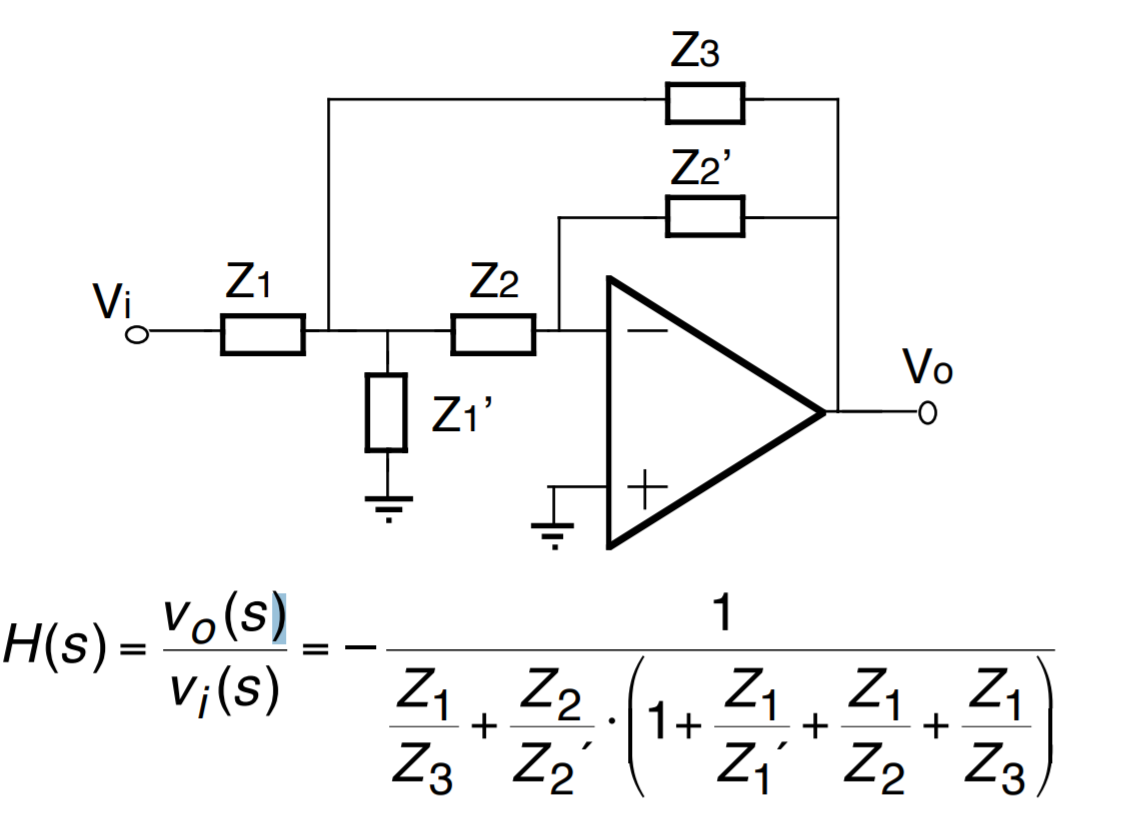
\includegraphics[scale=0.5]{imagenes/rauch_generico.png}
	\caption{Filtro Rauch para impedancias fijas}
	\label{fig:ej2_rauch_generico}
\end{figure}

 De él se pueden desprender filtros de orden dos como un pasa-altos, un pasa-bajos, pasabandas, etc. Intentaremos implementar etapas de tipo pasabandas para componer al filtro pasabandas.
  
 \section{Pasabandas Rauch}
 
 El filtro Rauch pasabandas está compuesto por los siguientes componentes:
 
 \begin{figure}[H]	% Rauch pasabandas
	\centering
	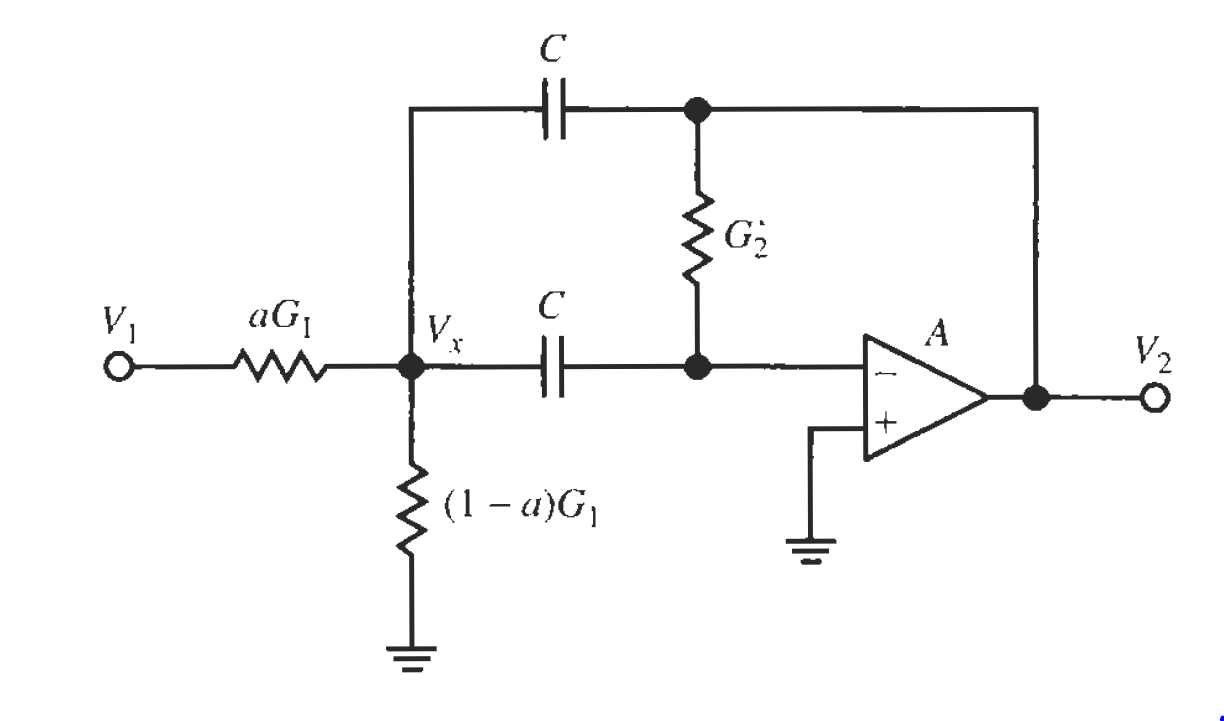
\includegraphics[scale=0.5]{imagenes/rauch_passband.png}
	\caption{Filtro Rauch pasabandas}
	\label{fig:ej2_rauch_passband}
	\end{figure}
	
	De aquí se deduce la función transferencia resultante en función de los componentes: \par
	
	\begin{centering}
	$H(s) = -\frac{C\, \mathrm{R_2}\, \mathrm{R_3}\, s}{\mathrm{R_1}\, \mathrm{R_2}\, \mathrm{R_3}\, C^2\, s^2 + 2\, 		\mathrm{R_1}\, \mathrm{R_3}\, C\, s + \mathrm{R_1} + \mathrm{R_3}}$
 \end{centering}
	\par Que puede ser mejor expresada como: \par
	\begin{centering}
	$H(s) = -\frac{1}{R_1\cdot c}\cdot \frac{s}{s^2 + \frac{2}{R_2\cdot C} \cdot s + \frac{R_1 + R_3}{R_1\cdot R_2 \cdot R_3 \cdot C^2}}$
	\end{centering}
	\par
	
	La ventaja del uso de este filtro es que permite obtener Q altos debido a las sensibilidades.\par
	
	\section{Implementación del filtro}
	
	\subsection{Plantilla}
	Se busca que el filtro cumpla con la plantilla con una máxima dispersión permitida del 1\%, por lo que se utilizarán resistencias SMD por su menor tolerancia. \par
	Usando un programa que permitía descomponer a un filtro en etapas y aproximarlo sólo con su plantilla, se obtuvieron los polos de la función de transferencia para la plantilla deseada. Como la consigna daba libertad en cuanto a los extremos que no son de la banda pasante y su correspondiente atenuación, se buscó que estos parámetros sean lo menos restrictivos posibles, ya que el orden del filtro estaba impuesto y condiciones más restrictivas impondrían necesariamente un orden mayor para el filtro.\par
	Se concluyó por lo tanto en definir un $f_a^+ = 900kHz$ y un $f_a^- = 5kHz$, con su correspondiente límite de atenuación mínima de $A_a = 50 dB$. Esta última cae dentro de los valores que hacen que el orden del filtro pasabajos normalizados sea 2.\par 
	Por otro lado, los datos de consigna arrojan una frecuencia central de pasabanda de $f_0^+ = 56kHz$, con su respectiva atenuación de banda pasante mínima $A_p  = 3 dB$. Al utilizar  estos datos, se obtienen Q muy altos para cualquier valor de $f_a^+$ y $f_a^-$, por lo que el filtro sería irrealizable a fines prácticos.\par
	 \begin{figure}[H]	% Qs muy altos con Ap = 3
	\centering
	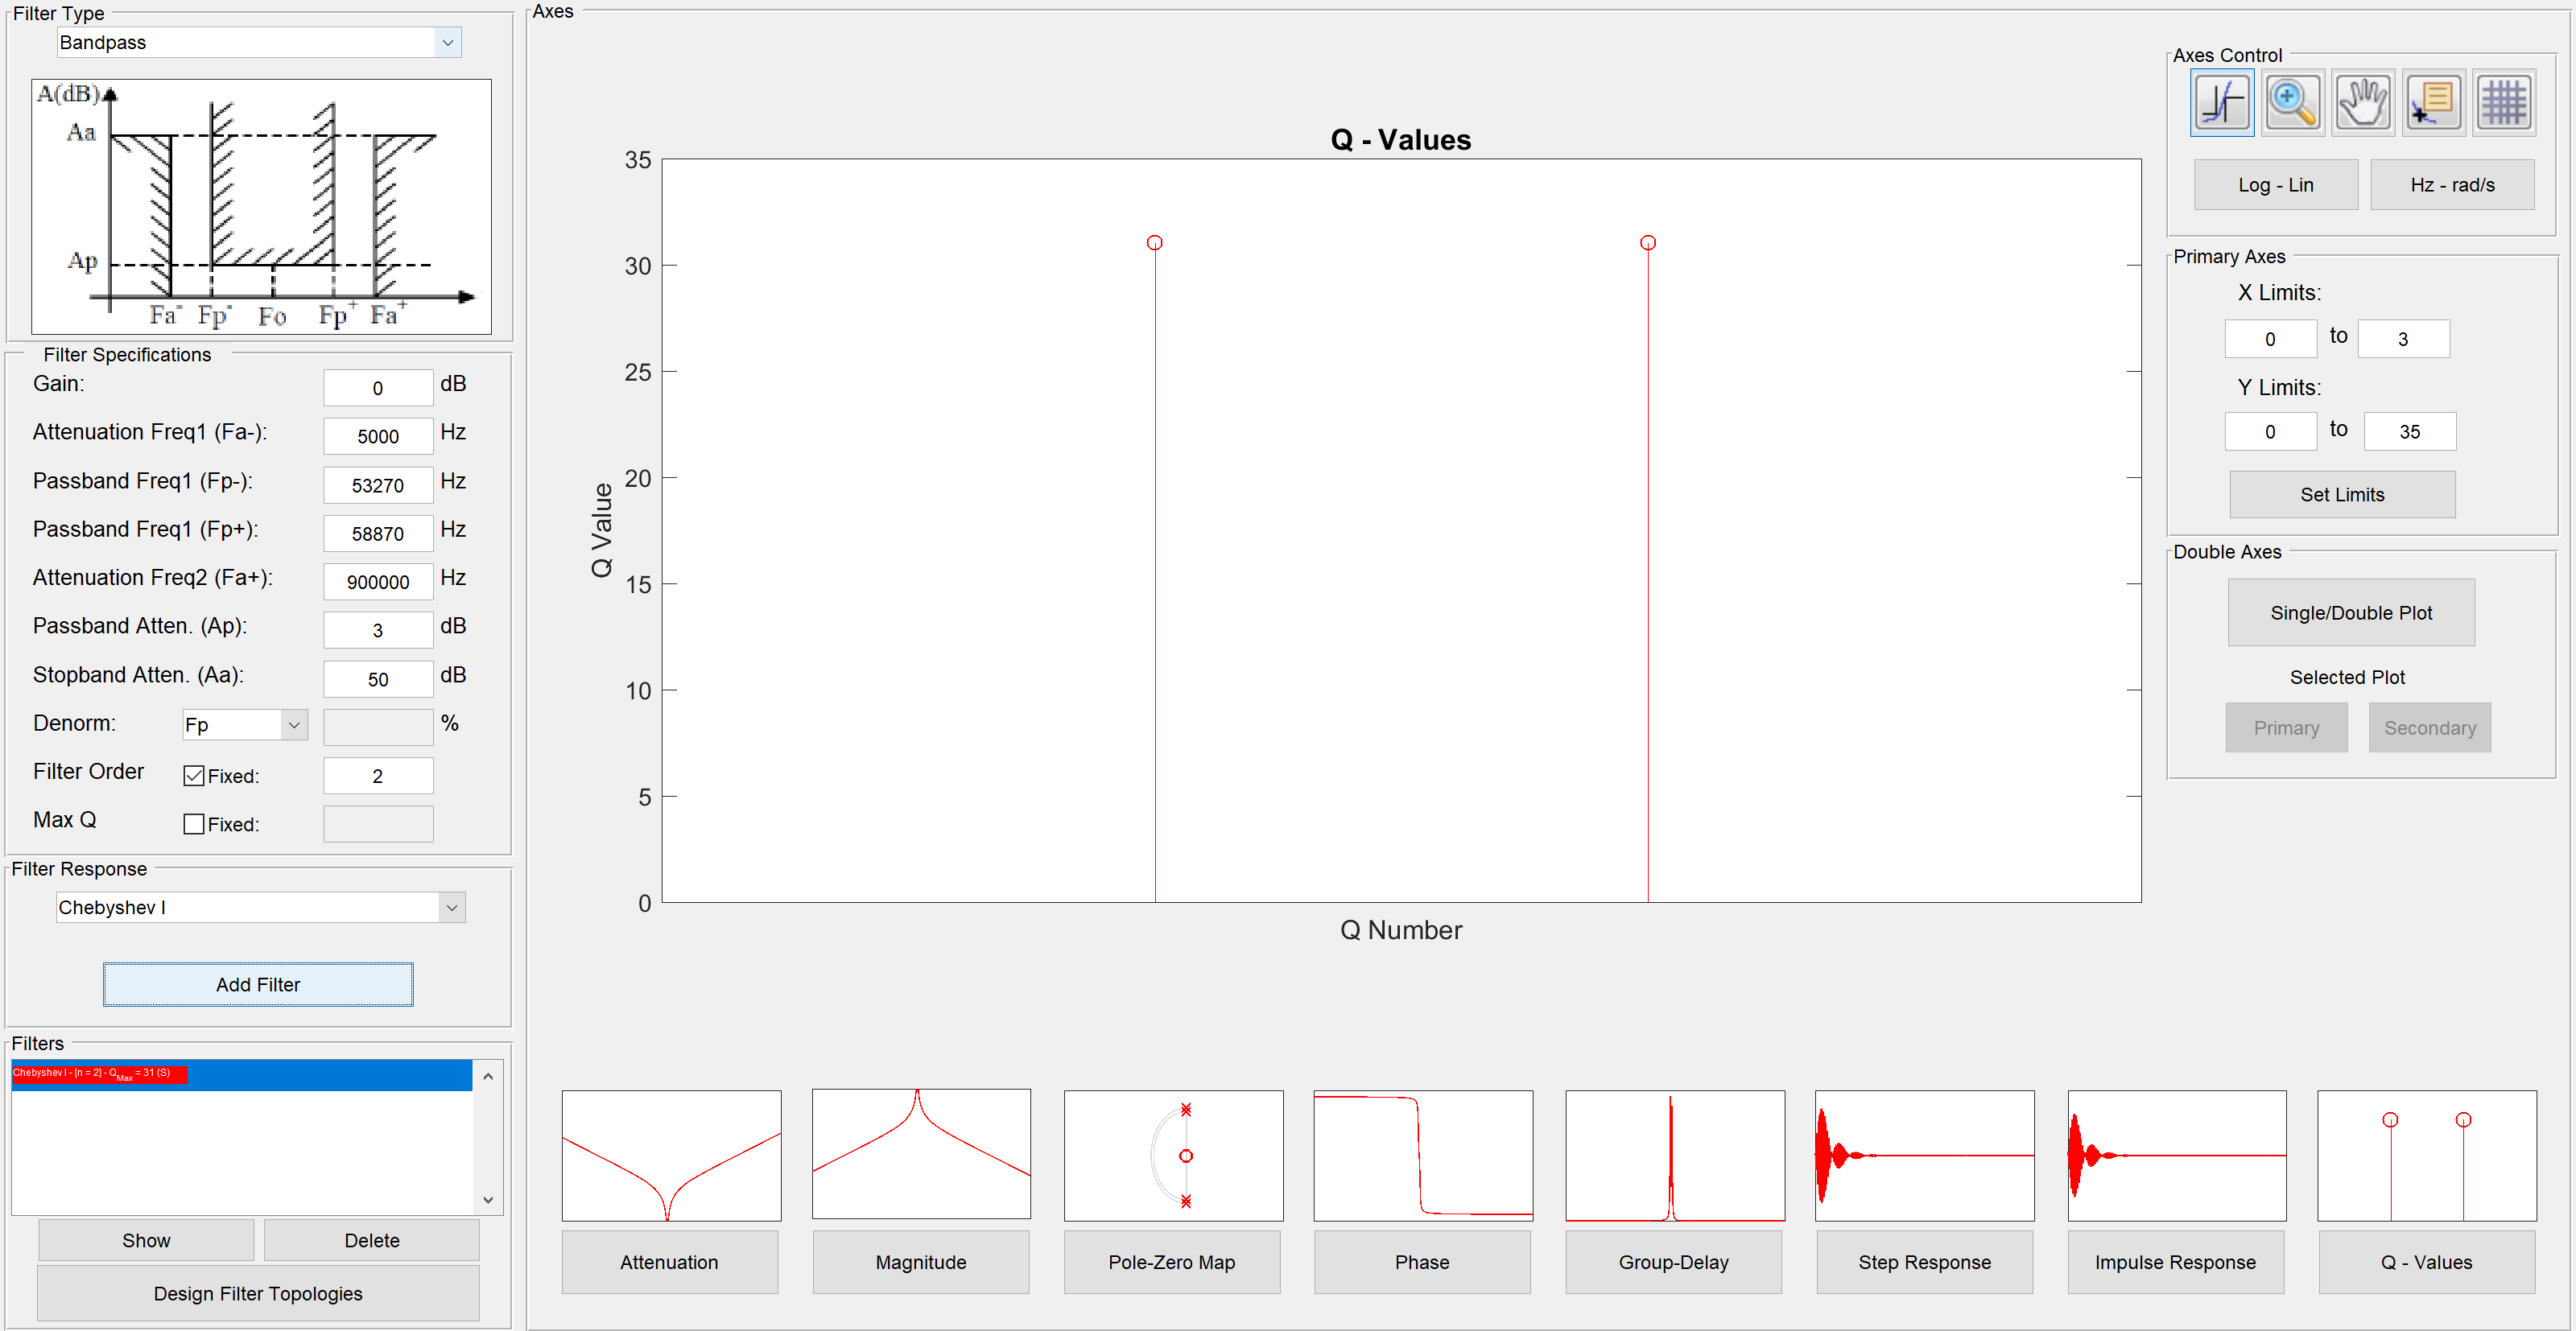
\includegraphics[scale=0.5]{imagenes/q_fallidos.png}
	\caption{Valores de Q para el filtro a implementar con Ap = 3dB}
	\label{fig:ej2_q_fallidos}
	\end{figure}
	Es por esta razón que se pide una menor atenuación mínima para la banda pasante, a modo de obtener menores valores de Q y aún así cumplir plantilla. Se elige esta atenuación de un valor de  $A_p  = 0.02 dB$.\par
	
	\subsection{Obtención de transferencia para la plantilla dada}
	
	Se obtiene mediante el programa los polos y ceros de la función de transferencia, que resultan ser: $f_1 = 50697 Hz$, $f_2 = 61857$,cada uno con un factor de calidad Q =5.42 y dos ceros en el origen.\par
	Esto puede ser implementado de diversas maneras en etapas. Como se pide utilizar un pasabandas rauch, las dos etapas de orden 2 a partir de las cuales se implemetará el filtro total de orden 4 serán las dos de tipo pasabandas, por lo que serán de la forma:
\begin{center}
$H(s) = \frac{A \cdot \frac{w_0}{Q}}{s^2 + w_0\cdot Q\cdot s + w_0^2}$
\end{center}
	\par
Donde A vale 3.35dB para ambas etapas. \par
Además, ambas etapas irán conectadas por un buffer para evitar que un circuito cargue al otro y así se corrompa la transferencia total.
		 \begin{figure}[H]	% polos y ceros determinados
	\centering
	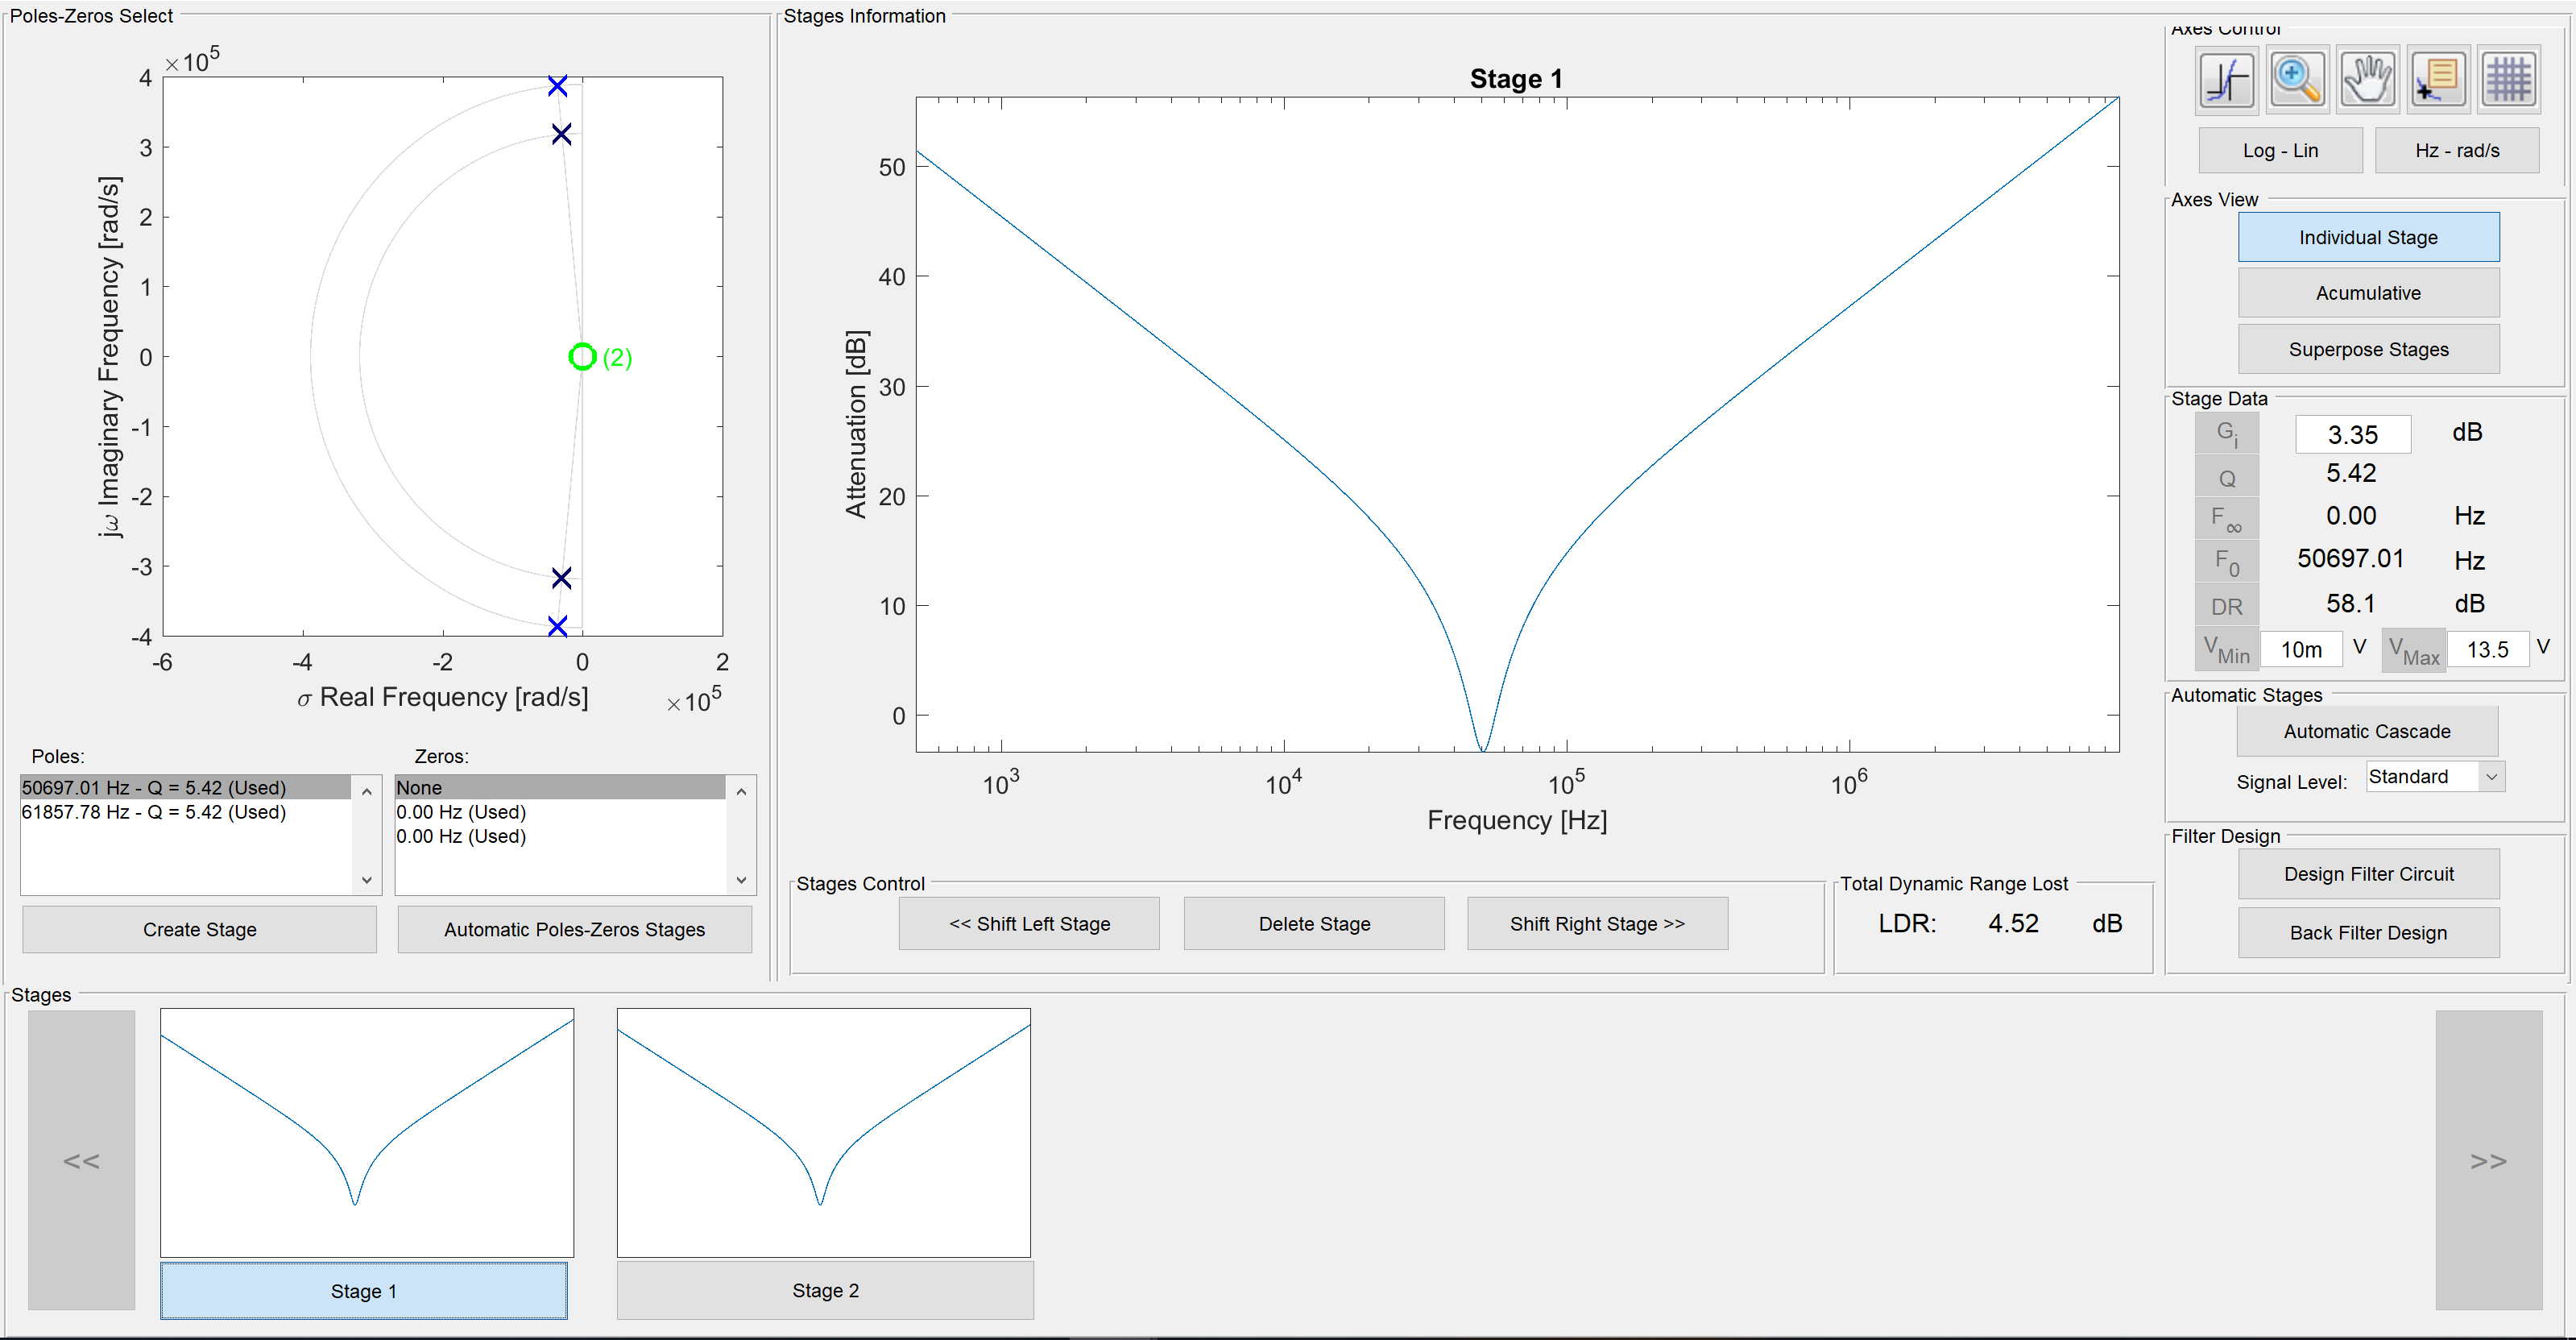
\includegraphics[scale=0.5]{imagenes/input_polos.png}
	\caption{Etapas determinadas con sus respectivos polos y ceros}
	\label{fig:ej2_input_polos}
	\end{figure}
	
 	Dados los valores de $w_0$, $A$ y $Q$ mencionados anteriormente, se procede a encontrar aquellos valores de componentes que logren implementar las etapas por separado. \par
 	Observando la transferencia del pasabajos Rauch, establecemos el vínculo entre los valores de los componentes y el parámetro de cada etapa, por lo que obtenermos: \par
 	\begin{itemize}
 		\item $w_0^2 = \frac{R_1 + R_3}{R_1\cdot R_2 \cdot R_3\cdot C^2}$
 		\item $\frac{w_0}{Q} = \frac{2}{R_2\cdot C}$
 		\item $A = -\frac{R_2}{2\cdot R_1}$
 	\end{itemize}
 	
 	Conociendo estos parámetros, podemos despejar los valores de los componentes como:
 	 	\begin{itemize}
 		\item $R_2 = 2\cdot \frac{Q}{w_0\cdot C}$
 		\item $R_1 = \frac{2\cdot H}{R_2}$
 		\item $R_3 = \frac{R_1}{w_0^2\cdot R_1\cdot R_2 \cdot C^2 - 1}$
 	\end{itemize}
 	
 	Y así, fijando el valor de los capacitores a $C = 1 nF$,  se obtiene el valor final de los componentes para la primera y la segunda etapa, de modo tal que: \par
 	 Etapa 1 $(f_1 = 50697 Hz)$:\par
 	 \par
 	\begin{itemize}
 		\item $C = 1 nF$
 		\item $R_2 = 34 k\ohm$
 		\item $R_1 = 11570 k\ohm$
 		\item $R_3 = 297$
 	\end{itemize}
 	 Etapa 2 $(f_2 = 61857)$: \par
 	 \par
 	  	\begin{itemize}
 		\item $C = 1 nF$
 		\item $R_2 = 27.9k\ohm$
 		\item $R_1 = 9.5 k\ohm$
 		\item $R_3 = 243$
 	\end{itemize}
 	
 	Luego se retocaron los valores de las resistencias $R_3$ para ambas etapas para que se obtuviesen mejores resultados al simular en Ltspice, obteniendo una mejor ganancia en la banda de paso y así mejorando el cumplimiento de la plantilla.\par
 	Para obtener una impedancia de entrada lo suficientemente grande, se dispuso de un buffer a la entrada, implementado con un opamp TL084 al igual que para el resto de los opamps utilizados. 
 	De aquí se presenta el circuito diseñado: \par
 	
 	 \section{Simulación}
		
 	 \section{Mediciones}
 	 
 	 \subsection{Análisis de Montecarlo}
 	 \subsection{}
\clearpage\newpage


\end{document}
